\chapter{Results}
\label{cha:results}

The techniques and procedures presented in the preceding chapter are all used to study an Ir(111) crystal with a graphene monolayer on top.

\section{Graphene on Ir(111)}

STM images of pure graphene on Ir(111) are shown in this section. Figure \ref{GrIr} shows images of graphene on Ir(111) in different sizes and, Figure \ref{GrIr1} shows a large image of a graphene monolayer covering the Ir(111) surface. Although the quality of the image is poor, which is seen as lines dragged across the surface, the moire pattern can be perceived as a pattern of small hexagonal structures. The blurred lines can be caused by the tip picking up an atom which momentarily change the LDOS of the tip, until the atom is dropped on the surface once again. The hexagonal structures, caused by the moiré pattern, are outlined in the top left of the image. Several step edges from the underlying Ir surface are also seen. Several line scans have been performed on these edges, which show that the height difference is 2Å $\pm$0.4Å. This value is consistent with the value of 0.22nm found in the literature.\cite{1367-2630-11-2-023006,coraux2008structural}\\
A high resolution image of Graphene on Ir(111) is shown in Figure \ref{GrIr2}. The moire pattern is very prominent in this figure, which once again is outlined as the blue hexagon, and the spacing between the individual sites in the moiré unit cell can be determined from a line scan. A line scan was drawn on Figure \ref{GrIr2}, and two points were positioned in the ATOP sites of the moire unit cell in order to obtain the moire periodicity. The moiré periodicity is 25.2 $\pm$ 0.4Å according to the literature.\cite{1367-2630-10-4-043033} This agrees with the length of 25.24 $\pm$ 1 Å measured from the line scan, which is seen on Figure \ref{linescan}. Typical defects of the graphene monolayer are seen in this figure, within the blue circle. These are likely to arise from carbon vacancies.\\
Figure \ref{GrIr3} shows a high quality image of the graphene monolayer on top of Ir(111). This image is a zoom in of the image shown in Figure \ref{GrIr2} corresponding to the dashed square. The smaller pattern mentioned before is much more visible in this image. The hexagonal pattern is the graphene monolayer on top of the iridium. The graphene hexagon is sketched as the blue hexagon and the moiré pattern seen on the two preceding figures is sketched as the dashed blue hexagon. The moiré unit cell is shown in the form of the blue rhombus, where the four dark corners correspond to the ATOP sites. The HCP and FCC sites lie at the corners of the dashed blue hexagon within the outlined moiré unit cell.

\begin{figure}[H]
\makebox[\textwidth][c]{
  \begin{subfigure}[b]{0.3\paperwidth}
    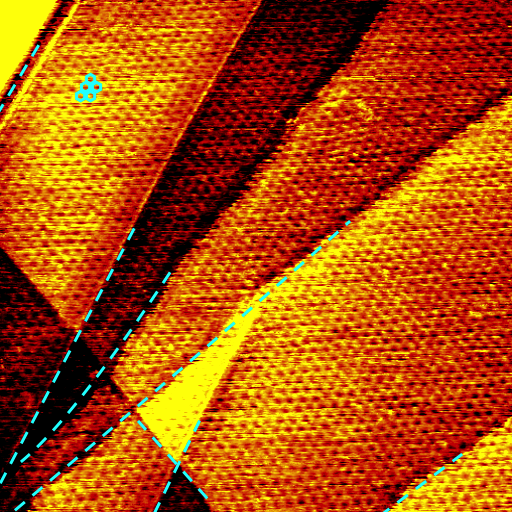
\includegraphics[height=\textwidth]{STMdata/FFT/2016-04-11_000_33.png}
    \caption{993x993 Å - I$_t$ = 0.690 nA, V$_t$ = 78.1 mV}
    \label{GrIr1}
  \end{subfigure}
  \begin{subfigure}[b]{0.3\paperwidth}
    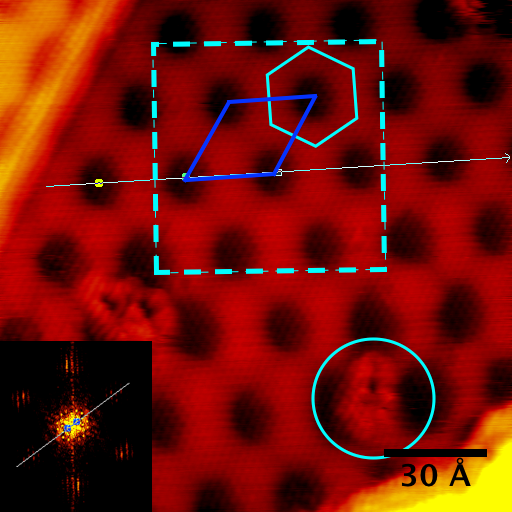
\includegraphics[height=\textwidth]{STMdata/FFT/2016-04-11_000_50.png}
    \caption{148x148 Å - I$_t$ = -0.890 nA, V$_t$ = -311.3 mV}
    \label{GrIr2}
  \end{subfigure}
  \begin{subfigure}[b]{0.3\paperwidth}
    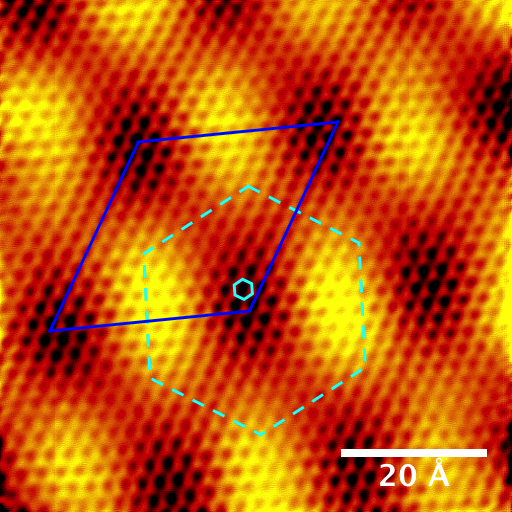
\includegraphics[height=\textwidth]{STMdata/FFT/2016-04-11_000_56.png}
    \caption{70x70 Å - I$_t$ = -0.910 nA, V$_t$ = -311.3 mV}
    \label{GrIr3}
  \end{subfigure}
  }
  \\
\makebox[\textwidth][c]{
  \begin{subfigure}[b]{0.7\paperwidth}
    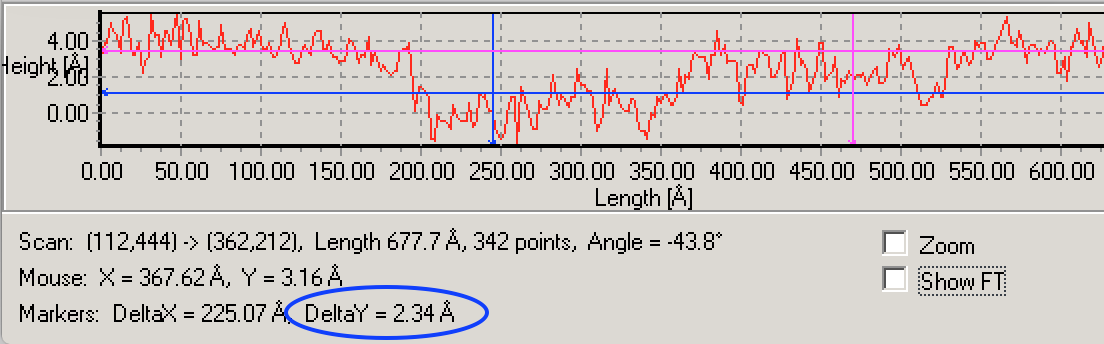
\includegraphics[width=\textwidth]{STMdata/FFT/linescanstep}
    \caption{Line profile of the line scan in Figure (a).}
    \label{linescanstep}
  \end{subfigure}
  \begin{subfigure}[b]{0.7\paperwidth}
    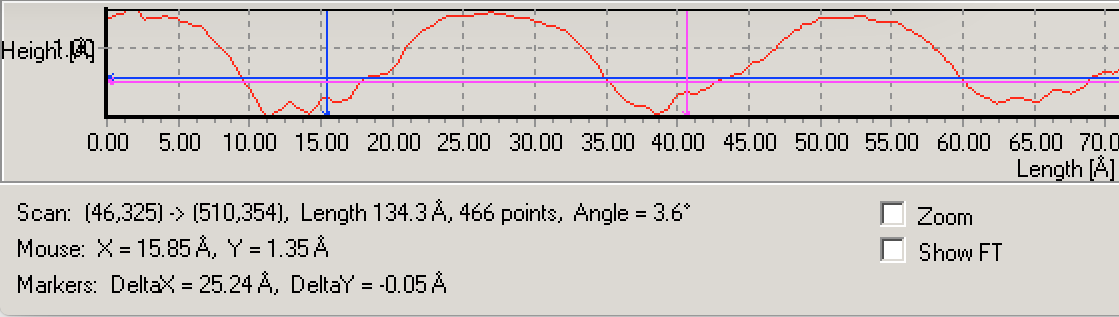
\includegraphics[width=\textwidth]{STMdata/FFT/Linescan}
    \caption{Line profile of the line scan in Figure (b).}
    \label{linescan}
  \end{subfigure}
}
\caption{Clean graphene on Ir(111). (c) is a zoom in of (b) which is shown as the dashed square.}
\label{GrIr}
\end{figure}

\section{D$_2$ on Graphene}

The following sections present the data from the dose of vibrationally excited molecules. The experiments aimed at determining the threshold temperature of the doser, regarding the hydrogenation of graphene. Hence, the temperature of the doser was varied in order to alter the flux of atoms from the doser, and thereby changing the number of hydrogen recombinations on the walls within the chamber as described in chapter \ref{theory}. Therefore, the data include dosages at temperatures of 1343\degree C, 1543\degree C, and 1745\degree C. The dosage time and D$_2$ pressure was identical in all off these doses, in order to ensure that the doser temperature was the only changed variable with an influence on the flux of atomic hydrogen. A dose at 1300\degree C was also performed. However, the STM broke, and therefore we did not get any images.


\subsection{Full Hydrogen Coverage}
A fully hydrogenated surface was used to create STM images. These images were compared to images of the short dosage experiments. The fully hydrogenated surface was made by filling the chamber with hydrogen at a pirani pressure of $6.8 \cdot 10^{-2}$mbar. This pressure should correspond to a chamber pressure of $5 \cdot 10^{-7}$mbar, according to the calibration, mentioned in chapter \ref{cha:procedure}. The ion gauge was turned off during the dose, in order to imitate the chamber conditions at short dosage periods. The dosage time was 60min. Figure \ref{D2:full} displays images of different scales. As seen from Figure \ref{full:1}, the sample is fully hydrogenated even at relative large areas of 949x949Å. Ring structures cover the surface of this image, instead of the moiré pattern observed in Figure \ref{GrIr1}. These structures can be more easily seen in Figure \ref{full:2}, which is a zoom in of Figure \ref{full:1}. The hydrogenated surface most often show ring shaped patterns in the form of structures with a bright rim and a darker center. By comparing Figures \ref{full:2} and \ref{GrIr2} it is obvious that the adsorption of hydrogen on the surface changes the LDOS. It is noticeable that the defects seen in Figure \ref{GrIr2} resemble the ring shaped structures seen in Figure \ref{D2:full}. Consequently, these defects might be caused by adsorbed hydrogen. Furthermore, some H-structures on the saturated surface seem to merge into a bigger structure, seen as the bone- and three point star shaped structures pointed out in Figure \ref{full:2}.
The sample was line scanned in order to check the periodicity of the pattern on the hydrogenated surface. The line scan is seen in Figure \ref{full:3}. and the related profile is shown in Figure \ref{linescan2}. The distance between the two points is 24.2 $\pm$1 Å. This value is very close to the expected periodicity of the moiré unit cell.\cite{1367-2630-11-2-023006}\\

\begin{figure}[H]
\makebox[\textwidth][c]{
  \begin{subfigure}[b]{0.3\paperwidth}
    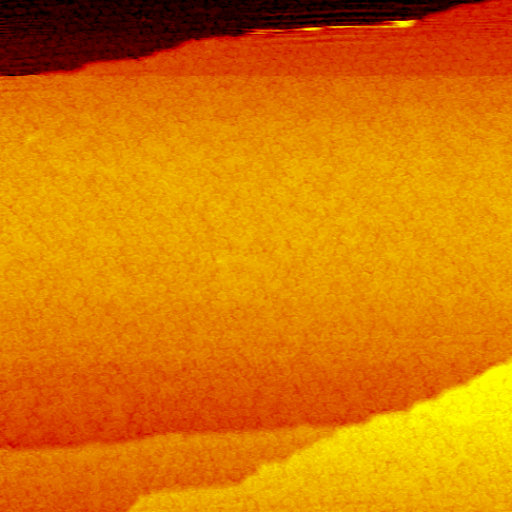
\includegraphics[height=\textwidth]{STMdata/FFT/2016-04-13_001_15.png}
    \caption{949x949 Å - I$_t$ = 0.860 nA, V$_t$ = 67.1 mV}
    \label{full:1}
  \end{subfigure}
  \begin{subfigure}[b]{0.3\paperwidth}
    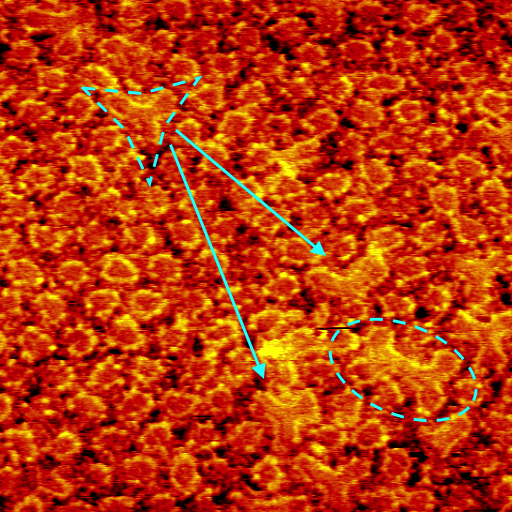
\includegraphics[height=\textwidth]{STMdata/FFT/2016-04-13_001_4.png}
    \caption{497x497 Å - I$_t$ = 0.850 nA, V$_t$ = 73.5 mV}
    \label{full:2}
  \end{subfigure}
  \begin{subfigure}[b]{0.3\paperwidth}
    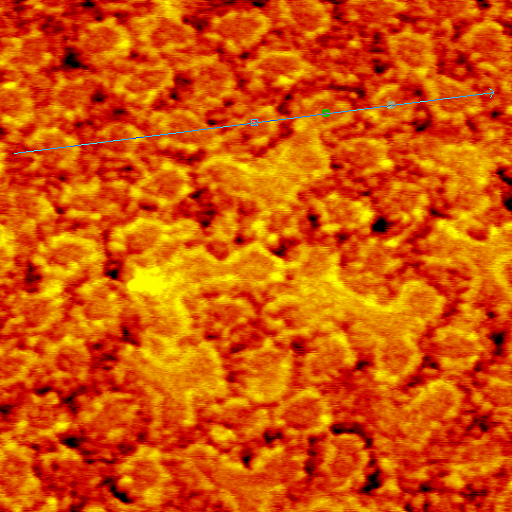
\includegraphics[height=\textwidth]{STMdata/FFT/2016-04-13_001_13.png}
    \caption{150x150 Å - I$_t$ = 0.850 nA, V$_t$ = 73.5 mV}
    \label{full:3}
  \end{subfigure}
}
\\
\makebox[\textwidth][c]{
\begin{subfigure}[b]{0.7\paperwidth}
  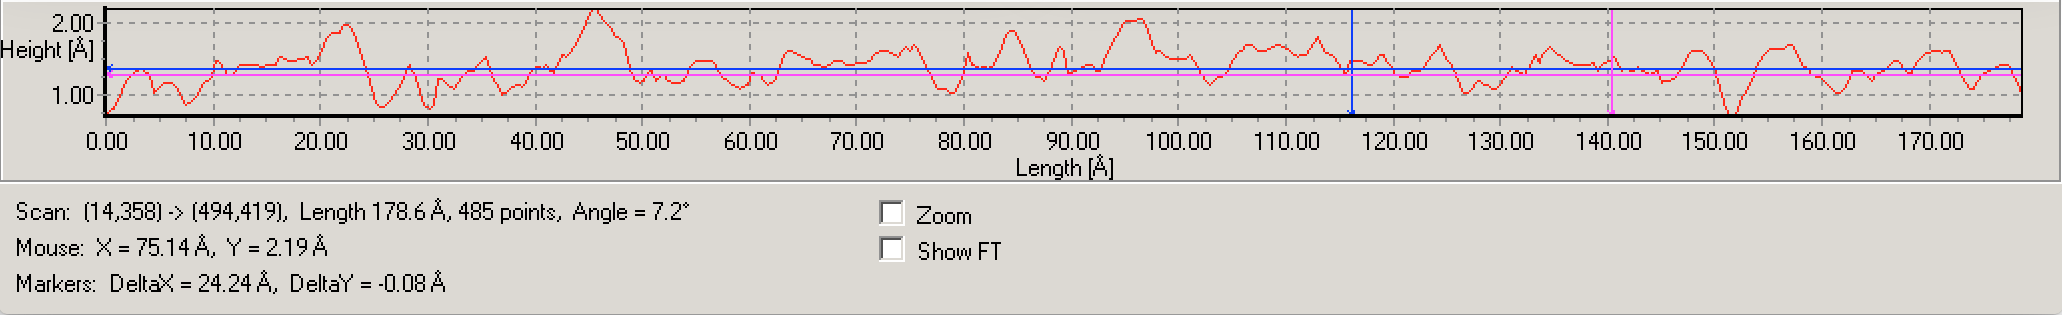
\includegraphics[width=\textwidth]{STMdata/FFT/LinescanfullH}
  \caption{Line profile of the linescan in figure (c).}
  \label{linescan2}
\end{subfigure}
}
\caption{Fully hydrogenated Gr/Ir(111) surface after 12h D$_2$ dosage. (c) is a zoom in on (b)}
\label{D2:full}
\end{figure}


\subsection{1745\degree C Dose}

This dosing was performed at a pirani pressure of $6.8 \cdot 10^{-2}$mbar, and with the doser set at a temperature of 1745\degree C. The dosage time was 20 min. The graphene was checked before dosing in order to reduce the number of defects as much as possible. Three images at different scales are shown in Figure \ref{D2:1745}. These images were taken immediately following the completion of the dosing. Comparing figures \ref{D2:17451} and \ref{full:1}, the surface in Figure \ref{D2:17451} is far from saturated, since the moiré pattern can be observed between areas in which the distinct ring structure of the hydrogenation is seen. It is also interesting that none of the hydrogenated sites melts together to form bigger structures, which indicates that this phenomenon happens as the surface becomes saturated.\\
In figure \ref{D2:1745} each moiré unit cell has been sketched with blue dashed lines. This shows that hydrogenation only happens at one site in the bottom left corner of the moiré unit cell. Earlier studies suggest that this is the FCC site in the moiré unit cell.\cite{Jakobunpublished} It is, however, seen that in some of the unit cells hydrogenation expands to the HCP site. This is illustrated by the dark blue circle.\\
Individual hydrogen atoms are not distinguishable from the STM images, and therefore the coverage is estimated as a percentage of the number of hydrogenated unit cells to the total number of unit cells. Figures \ref{D2:17452} and \ref{D2:17453} were used to calculate an estimate of the hydrogenation of the surface. The coverage on figure \ref{D2:17452} was calculated to 41\% and the coverage on figure \ref{D2:17453} was calculated to 29\%. This means that about one third of the unit cells is hydrogenated after a dosage of excited molecules for 20 min, at a chamber pressure of $5 \cdot 10^{-7}$mbar.

\begin{figure}[H]
\makebox[\textwidth][c]{
  \begin{subfigure}[b]{0.3\paperwidth}
    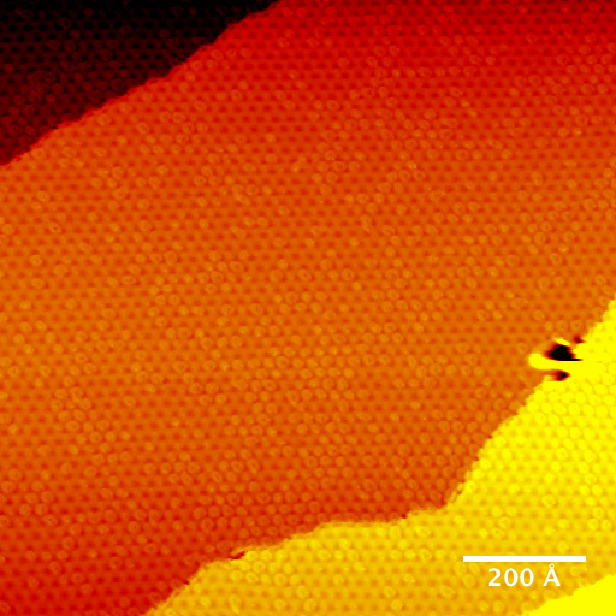
\includegraphics[height=\textwidth]{STMdata/FFT/2016-04-11_003_14.png}
    \caption{998x998 Å - I$_t$ = 1.060 nA, V$_t$ = 67.1 mV}
    \label{D2:17451}
  \end{subfigure}
  \begin{subfigure}[b]{0.3\paperwidth}
    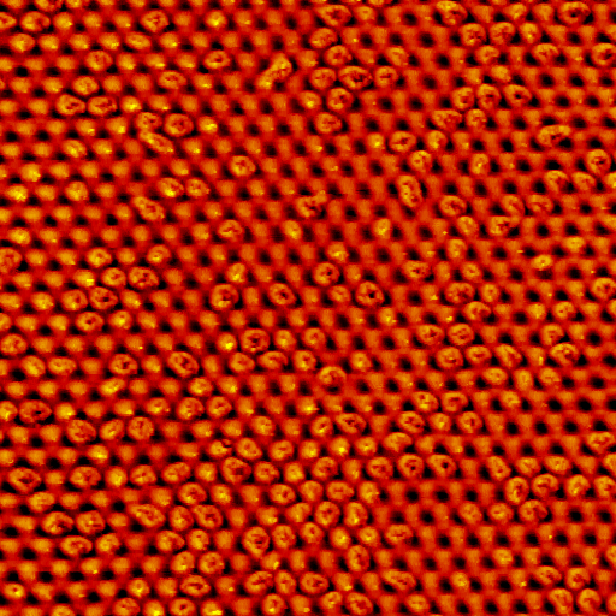
\includegraphics[height=\textwidth]{STMdata/FFT/2016-04-11_003_15.png}
    \caption{497x497 Å - I$_t$ = 1.080 nA, V$_t$ = 67.1 mV}
    \label{D2:17452}
  \end{subfigure}
  \begin{subfigure}[b]{0.3\paperwidth}
    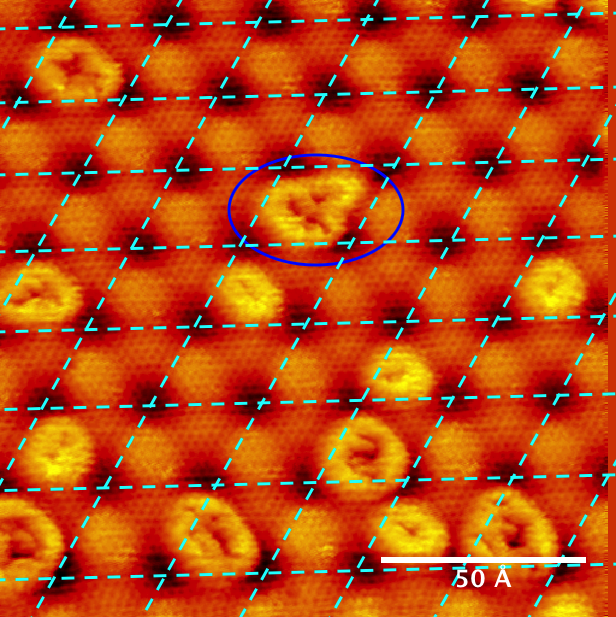
\includegraphics[height=\textwidth]{STMdata/FFT/2016-04-11_003_23.png}
    \caption{150x150 Å - I$_t$ = 1.090 nA, V$_t$ = 67.1 mV}
    \label{D2:17453}
  \end{subfigure}
}
\caption{Hydrogenated Gr/Ir surface after dose of D$_2$ at a doser temperature of 1745\degree C.}
\label{D2:1745}
\end{figure}

\subsection{1593\degree C Dose}

This dosing was performed at a pirani pressure of $6.8 \cdot 10^{-2}$mbar and a doser temperature of 1593\degree C. Again the dosing lasted 20 min. The images obtained after the dosing are shown in Figure \ref{D2:1593}. There is a remarkable resemblance between the pictures shown in Figures \ref{D2:1745} and \ref{D2:1593}. Again, both the ring shaped structure itself, and its shape are very similar to the ones observed earlier. It is seen that several ring structures are seen along the Ir step edge in Figure \ref{D2:15932}. The energy barrier is known to be less at step edges and dislocations \cite{Lineunpublished}, hence molecules excited to lower vibrational states might be able to hydrogenate the graphene in these regions. This could explain the hydrogenation along the step edge.\\
Figures \ref{D2:15931} and \ref{D2:15932} were used to calculate the coverage of hydrogenation, with values of 32\% and 25\%, respectively. These values are however very position dependant, and therefore they do not necessarily reflect the accurate coverage.

\begin{figure}[H]
\makebox[\textwidth][c]{
  \begin{subfigure}[b]{0.3\paperwidth}
    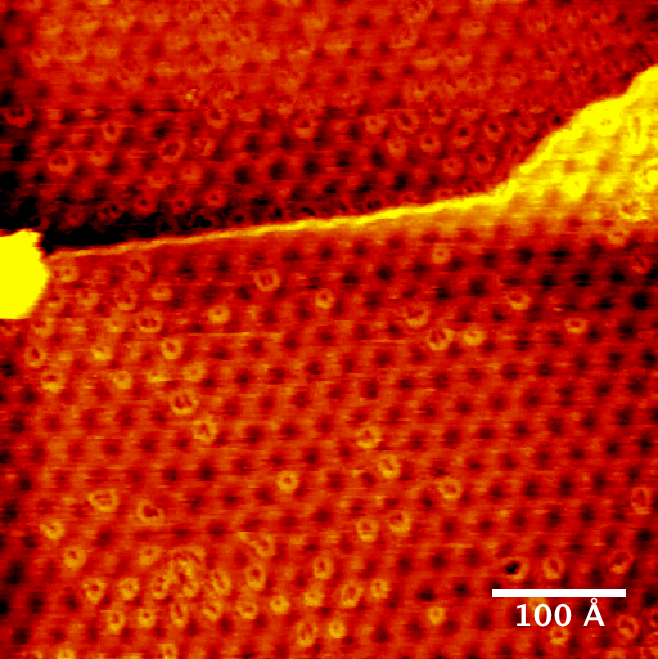
\includegraphics[height=\textwidth]{STMdata/FFT/2016-04-14_000_44.png}
    \caption{488x488 Å - I$_t$ = 0.900 nA, V$_t$ = 190.4 mV \qquad}
    \label{D2:15931}
  \end{subfigure}
  \begin{subfigure}[b]{0.3\paperwidth}
    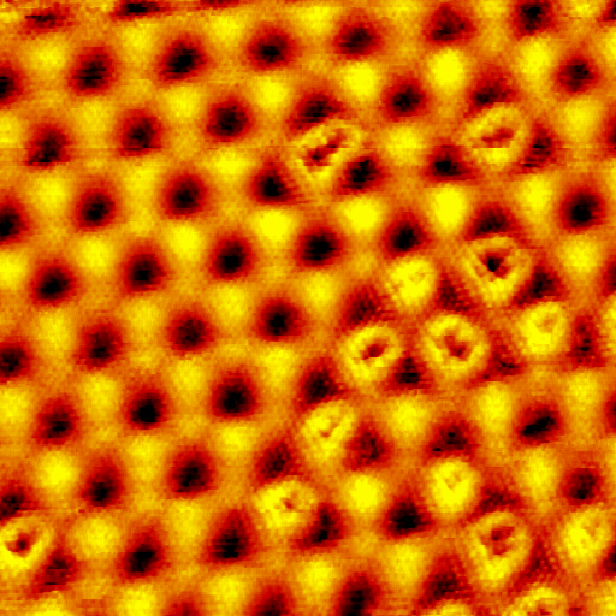
\includegraphics[height=\textwidth]{STMdata/FFT/2016-04-14_000_27.png}
    \caption{180x180Å - I$_t$ = 1.020 nA, V$_t$ = 190.4 mV \qquad}
    \label{D2:15932}
  \end{subfigure}
  \begin{subfigure}[b]{0.3\paperwidth}
    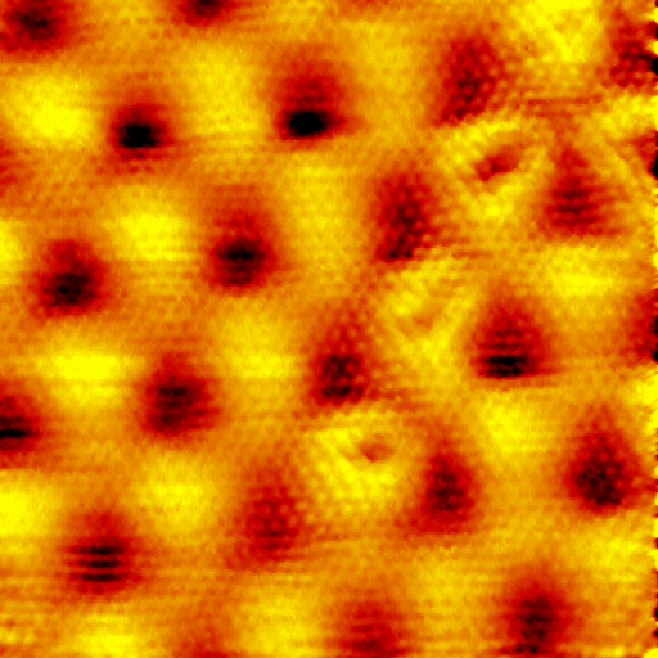
\includegraphics[height=\textwidth]{STMdata/FFT/2016-04-14_000_29.png}
    \caption{97x97 Å - I$_t$ = 1.020 nA, V$_t$ = 190.4 mV \qquad}
    \label{D2:15933}
  \end{subfigure}
}
\caption{Hydrogenated Gr/Ir surface after dose of D$_2$ at a doser temperature of 1593\degree C.}
\label{D2:1593}
\end{figure}

\subsection{1343\degree C Dose}

The pirani pressure was measured to $6.8 \cdot 10^{-2}$mbar, and the doser had a temperature of 1343\degree C during this dose. Hydrogen was dosed for 20 min. As seen in Figure \ref{D2:1340} several high quality pictures of the sample were taken. In Figure \ref{D2:13401} the observation of several ring shaped structures indicates that some hydrogen is adsorbed. As a zoom in is made such as the one in figure \ref{D2:13402} the defects differ from those seen earlier on figures \ref{D2:15932} and \ref{D2:17453}. The ring shaped structures are much smaller in diameter on figure \ref{D2:13402}, even though the scanning parameters are close to each other.\\
A high resolution image is seen in Figure \ref{D2:13403}, where the hexagonal graphene is highly visible. In this image it is clear that the graphene is defected, although it is unclear whether this is due to the presence of hydrogen. It should be noted that the graphene had defects before the dose was initiated. The abundance of these defects was indistinguishable, when comparing before and after the dose. Therefore it is not possible to conclude whether the threshold temperature of the hydrogen adsorption from excited molecules lies at 1340\degree C. It is however very likely that no hydrogen is adsorbed since these defects resemble carbon vacancies as seen in the litterature.\cite{1367-2630-11-2-023006}\\
In order to investigate the threshold temperature further, it would be rational to conduct TPD measurements of the sample after hydrogen dosage at 1343 \degree C. By doing so it would become clear whether any hydrogen is adsorbed on the graphene. \\
 It is also seen that the shape of the sites in the moiré unit cell looks different than earlier although both pictures are from the same scan session. This is due to a tip effect, where the LDOS of the tip has probably changed, which affects the tunnelling current. This  might happen if the tip picks up an atom from the surface, or if the physical dimensions of the tip changes after a tip treatment.


\begin{figure}[H]
\makebox[\textwidth][c]{
  \begin{subfigure}[b]{0.3\paperwidth}
    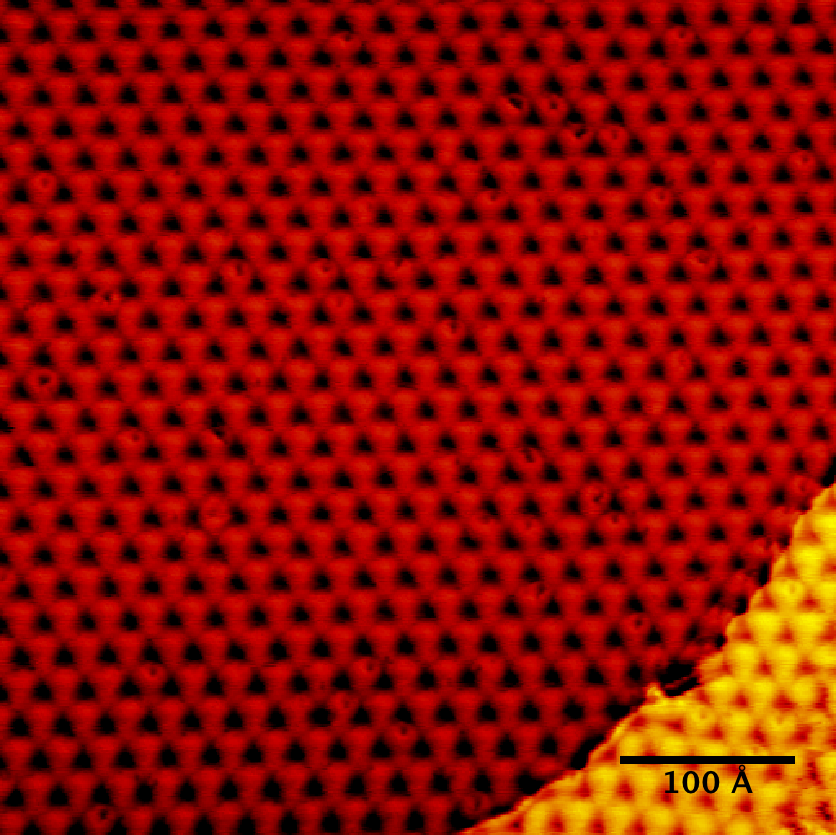
\includegraphics[height=\textwidth]{STMdata/FFT/2016-04-16_001_50_26.png}
    \caption{477x477 Å - I$_t$ = 0.820 nA, V$_t$ = 20.1 mV }
    \label{D2:13401}
  \end{subfigure}
  \begin{subfigure}[b]{0.3\paperwidth}
    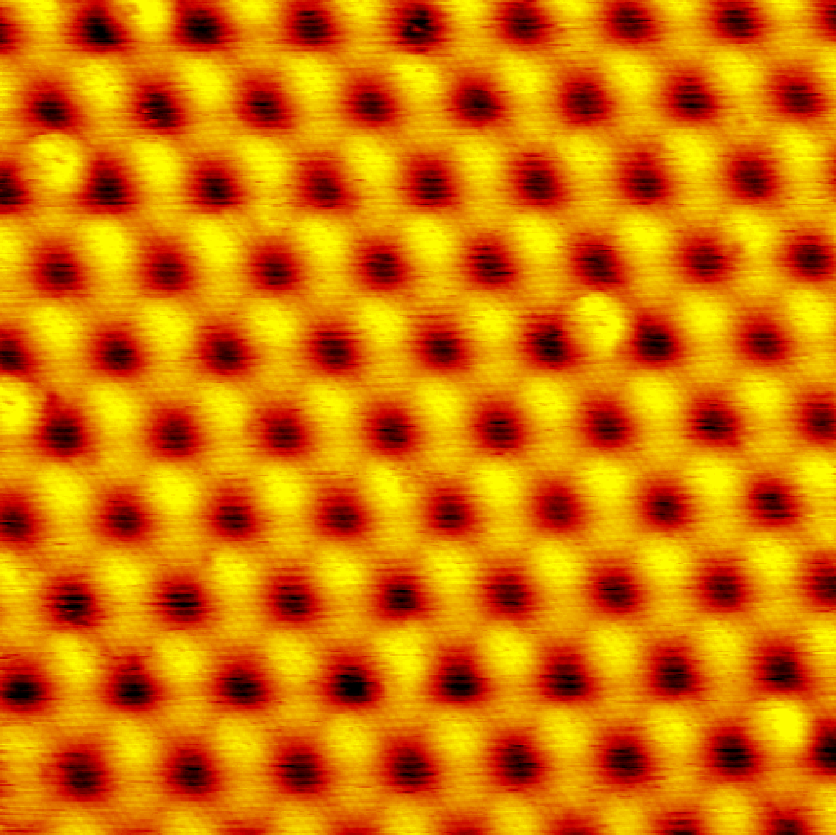
\includegraphics[height=\textwidth]{STMdata/FFT/2016-04-16_001_50_8.png}
    \caption{192x192Å - I$_t$ = 0.830 nA, V$_t$ = 55.8 mV }
    \label{D2:13402}
  \end{subfigure}
  \begin{subfigure}[b]{0.3\paperwidth}
    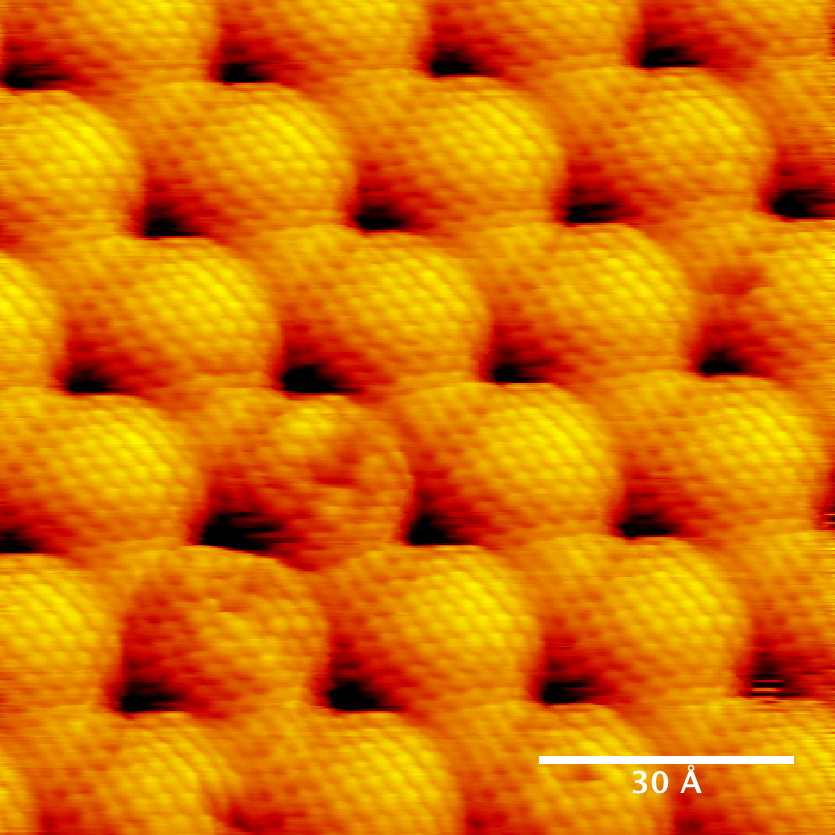
\includegraphics[height=\textwidth]{STMdata/FFT/2016-04-16_001_50_15.png}
    \caption{98x98 Å - I$_t$ = 0.820 nA, V$_t$ = 20.1 mV \qquad \qquad}
    \label{D2:13403}
  \end{subfigure}
}
\caption{Hydrogenated Gr/Ir surface after dose of D$_2$ at a doser temperature of 1343\degree C.}
\label{D2:1340}
\end{figure}


\section{TPD measurements}
In the following sections, TPD measurements from graphene on Ir(111) exposed to both vibrationally excited molecules and atomic hydrogen are compared.

\subsection{Atomic and molecular D2 - single layered sample}

In Figure \ref{TPD:all} below, the data from the TPD is gathered in two different figures. TPD measurements were made following doses of both vibrationally excited molecules and atomic hydrogen on the new sample with a fresh monolayer of graphene on Ir(111). Figure \ref{TPD:D2} shows the TPD data following a 60 min dose of D$_2$ at a chamber pressure of $5\cdot 10^{-7}$mbar and a doser temperature of 1740\degree C. The data is sketched in Figure \ref{TPD:D} following a 60 min dose of hydrogen atoms at a chamber pressure of $5\cdot 10^{-7}$mbar and a doser temperature of 1740\degree C.\\
After dosage of excited molecules a single peak is observed which is seen in Figure \ref{TPD:D2}. A big peak is seen after the main peak, at a temperature of about 800K. This is due to a temperature spike caused by the Eurotherm temperature controller, which was poorly calibrated as explained in chapter \ref{cha:procedure}. Noticeable fluctuations, caused by this problem, are also seen in Figure \ref{TPD:D}. This dataset was gathered during the same chamber and sample conditions as the blue graph in Figure \ref{TPD:D2}.\\
The temperature at the peak was found by the procedure described in chapter \ref{cha:procedure}. The single peak in Figure \ref{TPD:D2} must correspond to the hydrogen adsorbed on the HCP and FCC sites in the moiré unit cell. This statement is supported by the preceding STM pictures that show no sign of hydrogen dimers in the ATOP sites. The temperature of this peak was found for 6 datasets in all, and the values of these are shown in Table \ref{edes}. The calculated energies of desorption by the Redhead method are all around 2 eV. This value is close to the calculated average hydrogen binding energy of 2.20 eV\cite{balog2013controlling} within a graphane like island. Further calculations of the adsorption barrier is made in recent research. Here it is found that the initial hydrogen molecule percieves an adsorption barrier of 3eV. Hereafter the adsorption barrier undergoes a reduction of 1 eV due to the distortion of the graphene from the sp$^2$ to sp$^3$ rehybridization.\\
\begin{table}
  \centering
  \makebox[\textwidth][c]{
  \begin{tabular}{c|c|c|c|c|c|c}
    Sample & fig.\ref{TPD:D2} blue & fig.\ref{TPD:D22} green & fig.\ref{TPD:D} blue & fig.\ref{TPD:D2} green & fig.\ref{TPD:bilayer} green & fig.\ref{TPD:bilayer} red\\
    \hline
    Peak T [K] & 724.8 & 698.4 & 694.0 & 709.1 & 739.1 & 753.4\\
     E$_{des}^{Redhead}$ [eV] & 2.1$\pm$0.4 & 2.0$\pm$0.4 & 2.0$\pm$0.4 & 2.0$\pm$0.4 & 2.1$\pm$0.4 & 2.1$\pm$0.4
  \end{tabular}}
  \caption{}
  \label{edes}
\end{table}

Another peak appears when observing the data after the dose with atomic hydrogen, as seen in Figure \ref{TPD:D}. Hydrogen desorbs from the sample at two different desorption energies, which is seen from the two peaks. The temperature of these peaks were found by the same procedures as earlier, and the values were found to be 550.4K and 694.0K. The lower peak suggests that a different type of Gr-H bond is present. The most plausible explanation is the presence of hydrogen dimers on the ATOP site of the moiré unit cell. The presence of these are supported by the litterature, with DFT calculations.\cite{balog2013controlling} Earlier TPD measurements of deuterium dosed on highly ordered pyrolytic graphite (HOPG) have shown that dimer peaks appear at 445K and 560K.\cite{hornekaer2006metastable} These values are in correspondence with the peak in Figure \ref{TPD:D}. However, through discussions with the lab supervisor it was suggested that the peak intensity in this figure is too high to only stem from dimers. Therefore hydrogen must desorb from another source within the chamber during the TPD measurements. It is reasonable that this contribution come from the desorption of hydrogen from the Tantalum sample holder.

\begin{figure}
  \centering
  \begin{subfigure}[b]{0.45\textwidth}
    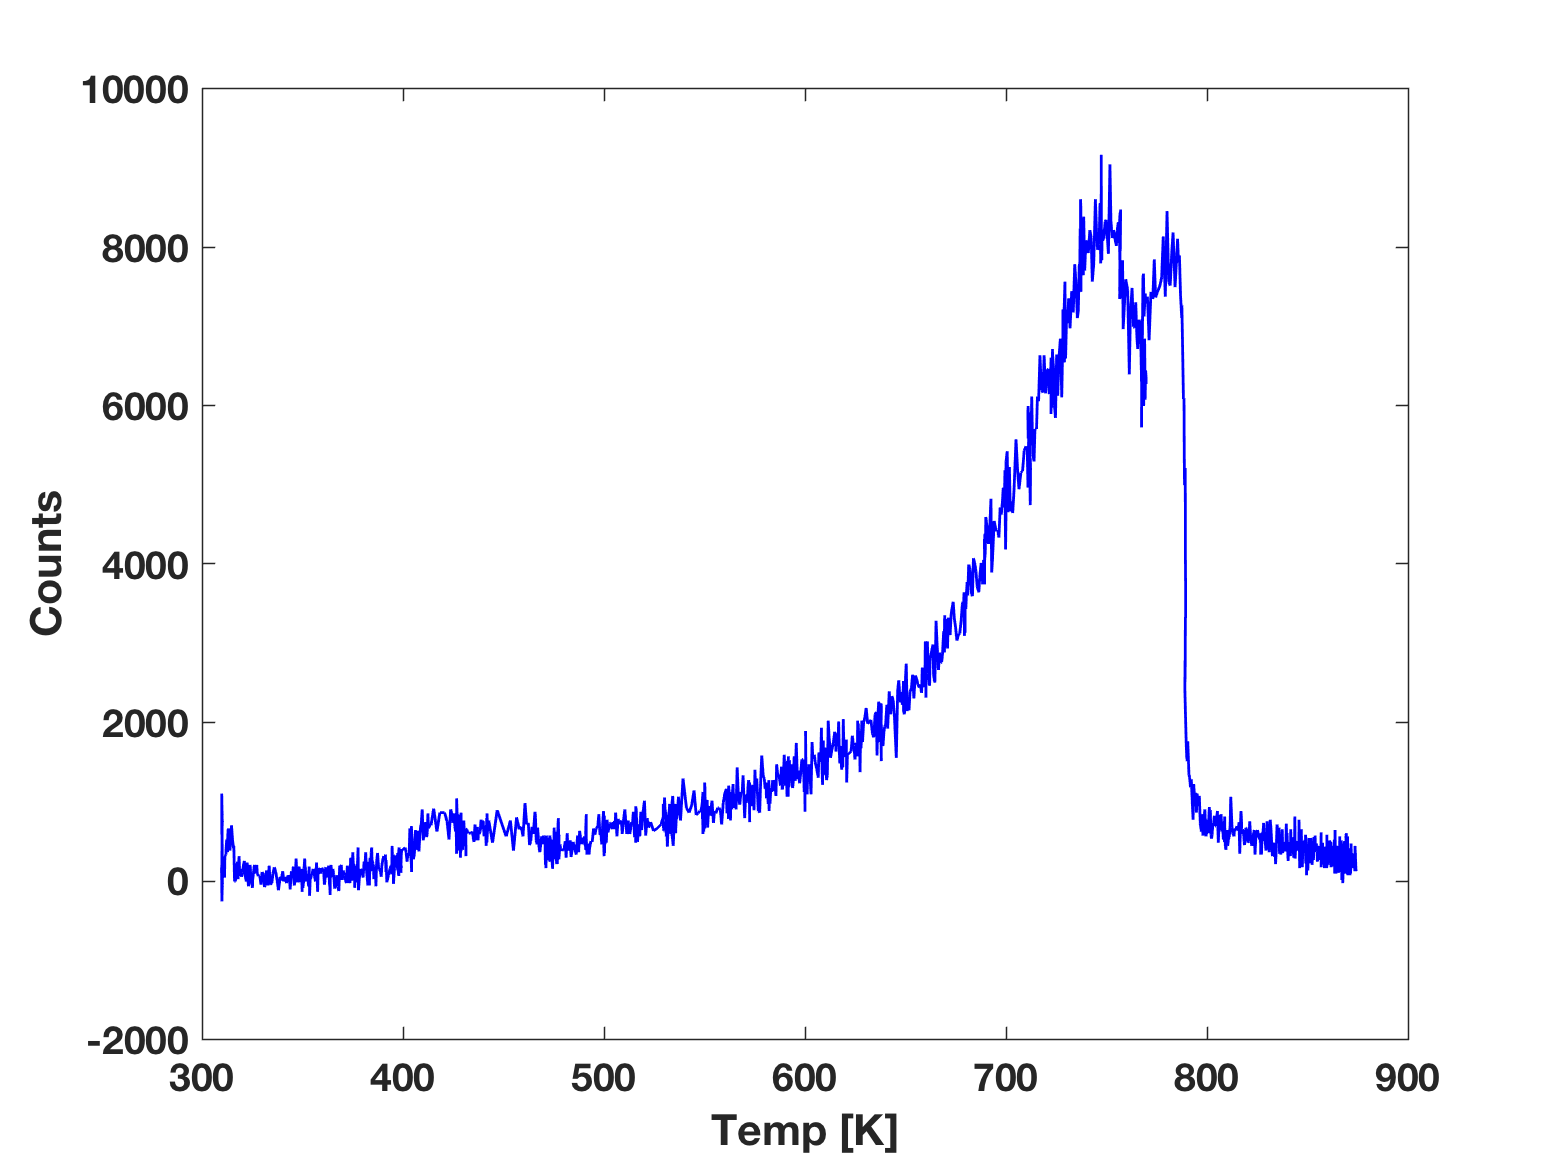
\includegraphics[width=\textwidth]{TPD/050516IrSorenD2dose1hour2temp.png}
    \caption{}
    \label{TPD:D2}
  \end{subfigure}\hspace{0.5cm}
  \begin{subfigure}[b]{0.45\textwidth}
    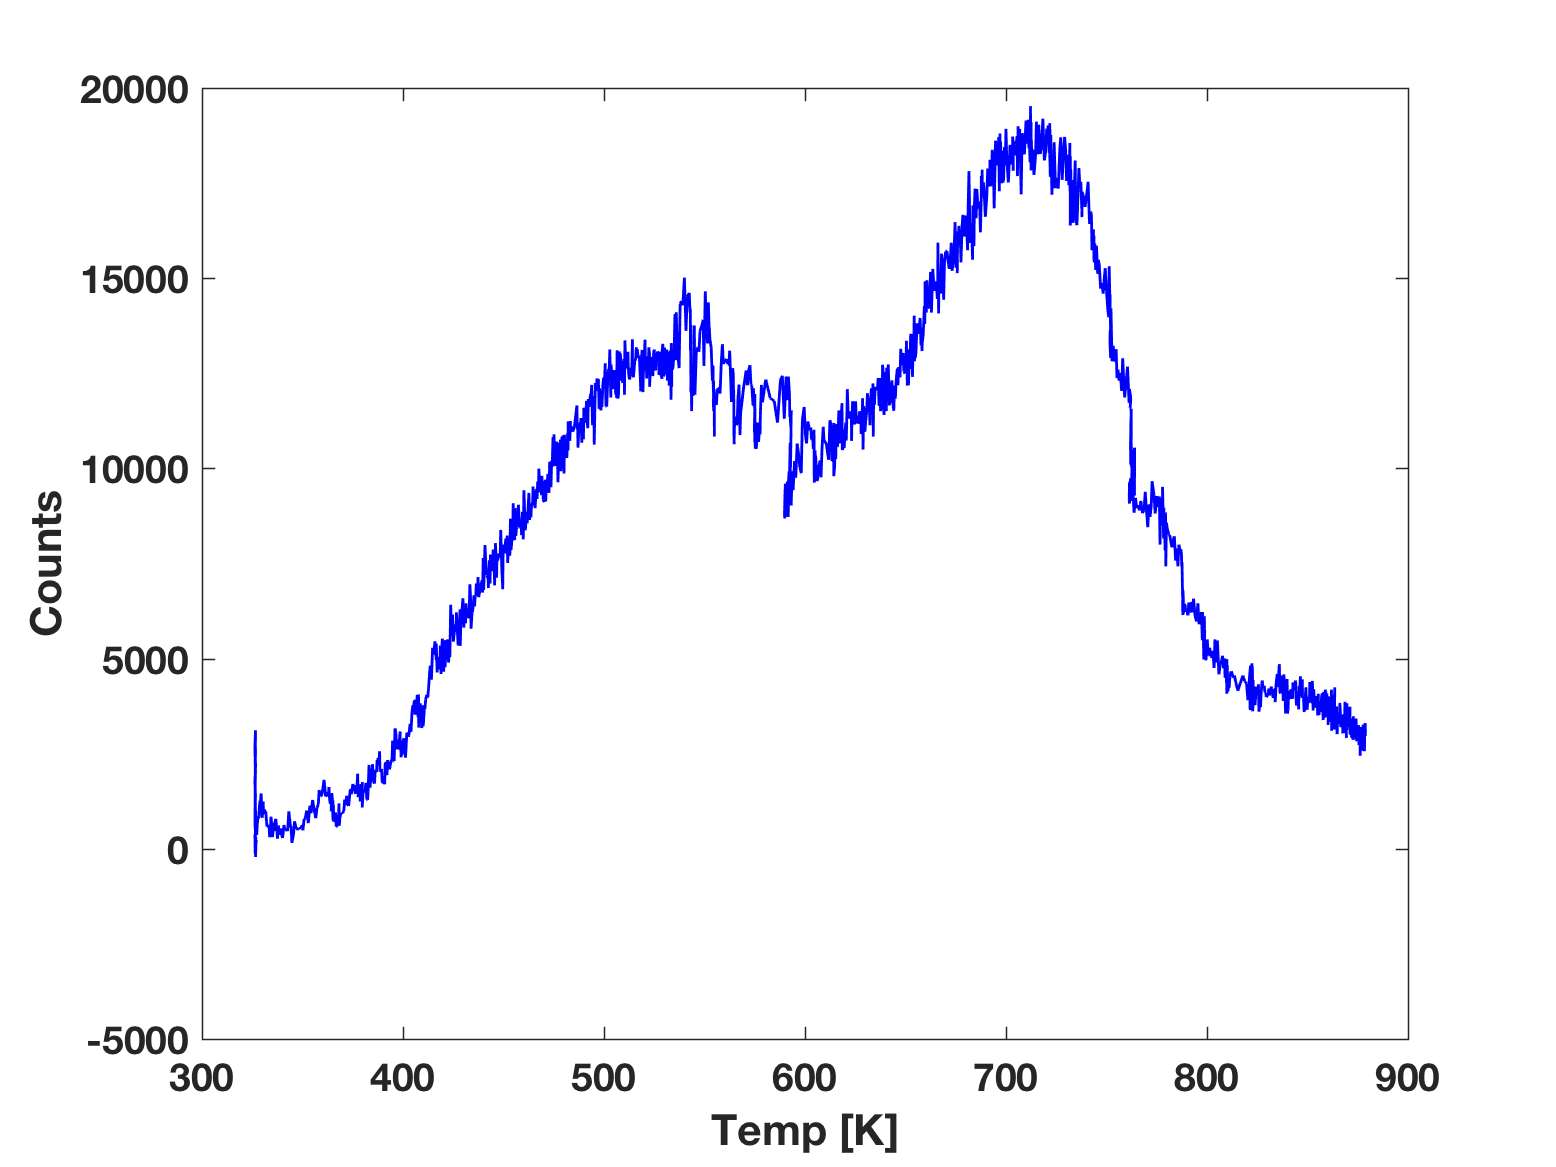
\includegraphics[width=\textwidth]{TPD/050516IrSorenDdose1hour2temp.png}
    \caption{}
    \label{TPD:D}
  \end{subfigure}
  \caption{TPD measurements following doses of D$_2$ and atomic hydrogen. (a) shows the graph following a 1 hour D$_2$ dose on graphene on Ir(111) with a doser temperature of 1740 \degree C and a chamber pressure of $5\cdot 10^{-7}$mbar. and (b) shows the graph following a 1 hour D dose on graphene on Ir(111) with a doser temperature of 1740 \degree C and a chamber pressure of $5\cdot 10^{-7}$mbar.}
  \label{TPD:all}
\end{figure}

\section{Graphene bilayered sample}

As a further study of the adsorption of hydrogen on Gr/Ir, patches of graphene bilayers were grown on the sample by annealing in ethylene for a long period of time. The sample was investigated with several techniques, and the results are presented in the following sections.

\subsection{TPD of bilayered sample}
TPD measurements were conducted on the sample before and after the long anneal. The red graph in figure \ref{TPD:bilayer} is the TPD results following a 60 min dose of D$_2$ at a chamber pressure of $1.04\cdot10^{-6}$mbar and with a doser temperature of 1740\degree C. \\
The green graph corresponds to the sample after bilayers supposedly were grown. Bilayers were grown by exposing the sample to ethylene at a pressure of $1\cdot 10^{-6}$mbar for 60 min, while the sample was heated to 990\degree C. The sample was dosed with atomic hydrogen at a chamber pressure of $1.04\cdot 10^{-6}$mbar and with a doser temperature of 1740K as well as before. It is seen that the peak value this time is around 6.000, which means that the increased amount of bilayers reduce the amount of hydrogen on the surface by a significant amount. This suggests that hydrogen is not adsorbed on the bilayered graphene. This theory is supported by the STM pictures below.\\
It should be noted that only two datasets were gathered from this experiment. The peak intensity from the TPD measurements tends to vary slightly and hence the amount of bilayers grown on the sample might not be perfectly related to the drop in peak intensity.
\begin{figure}[H]
  \centering
  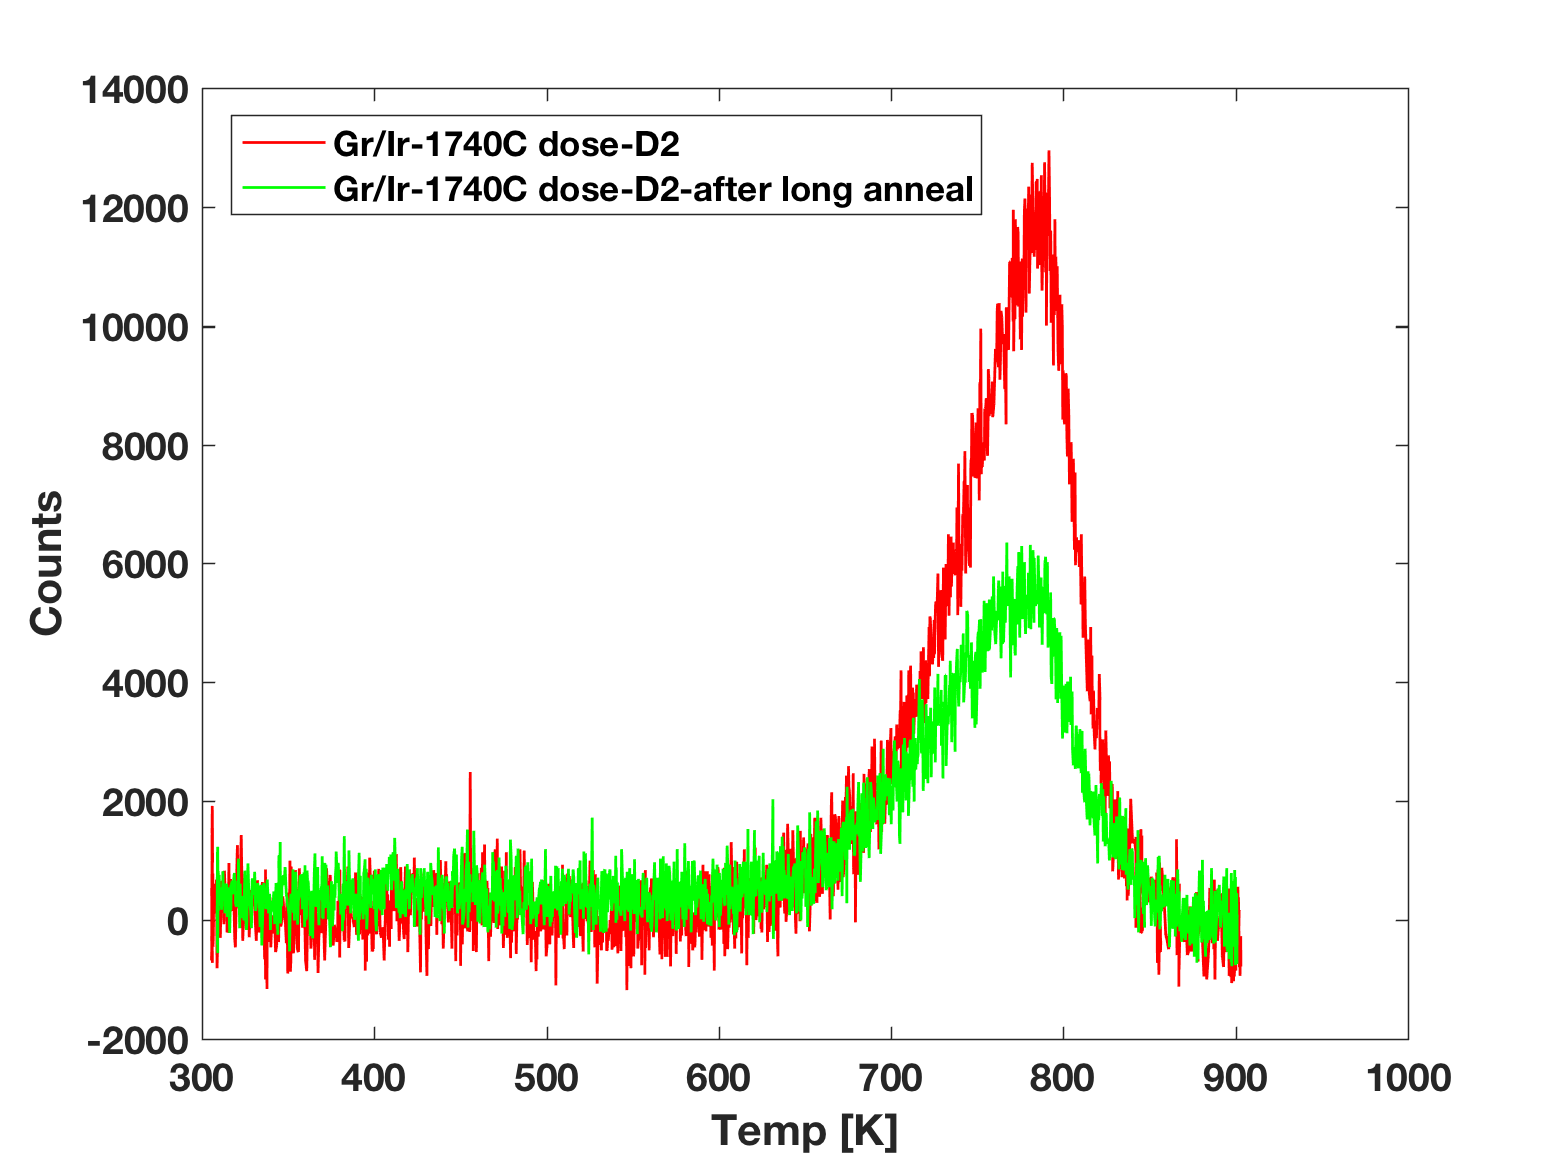
\includegraphics[width=0.6\textwidth]{TPD/GrIr1740CD2longannealtemp.png}
  \caption{TPD measurements after doses of D$_2$ at a pressure of $1.04\cdot10^{-6}$ and a doser T of 1740\degree C. The red graph is prior to a 60 min growth of bilayers where the 990\degree C sample was exposed to ethylene for 60 min at a pressure of $1\cdot10^{-6}$mbar}
  \label{TPD:bilayer}
\end{figure}



\begin{figure}
  \centering
  \begin{subfigure}[b]{0.45\textwidth}
    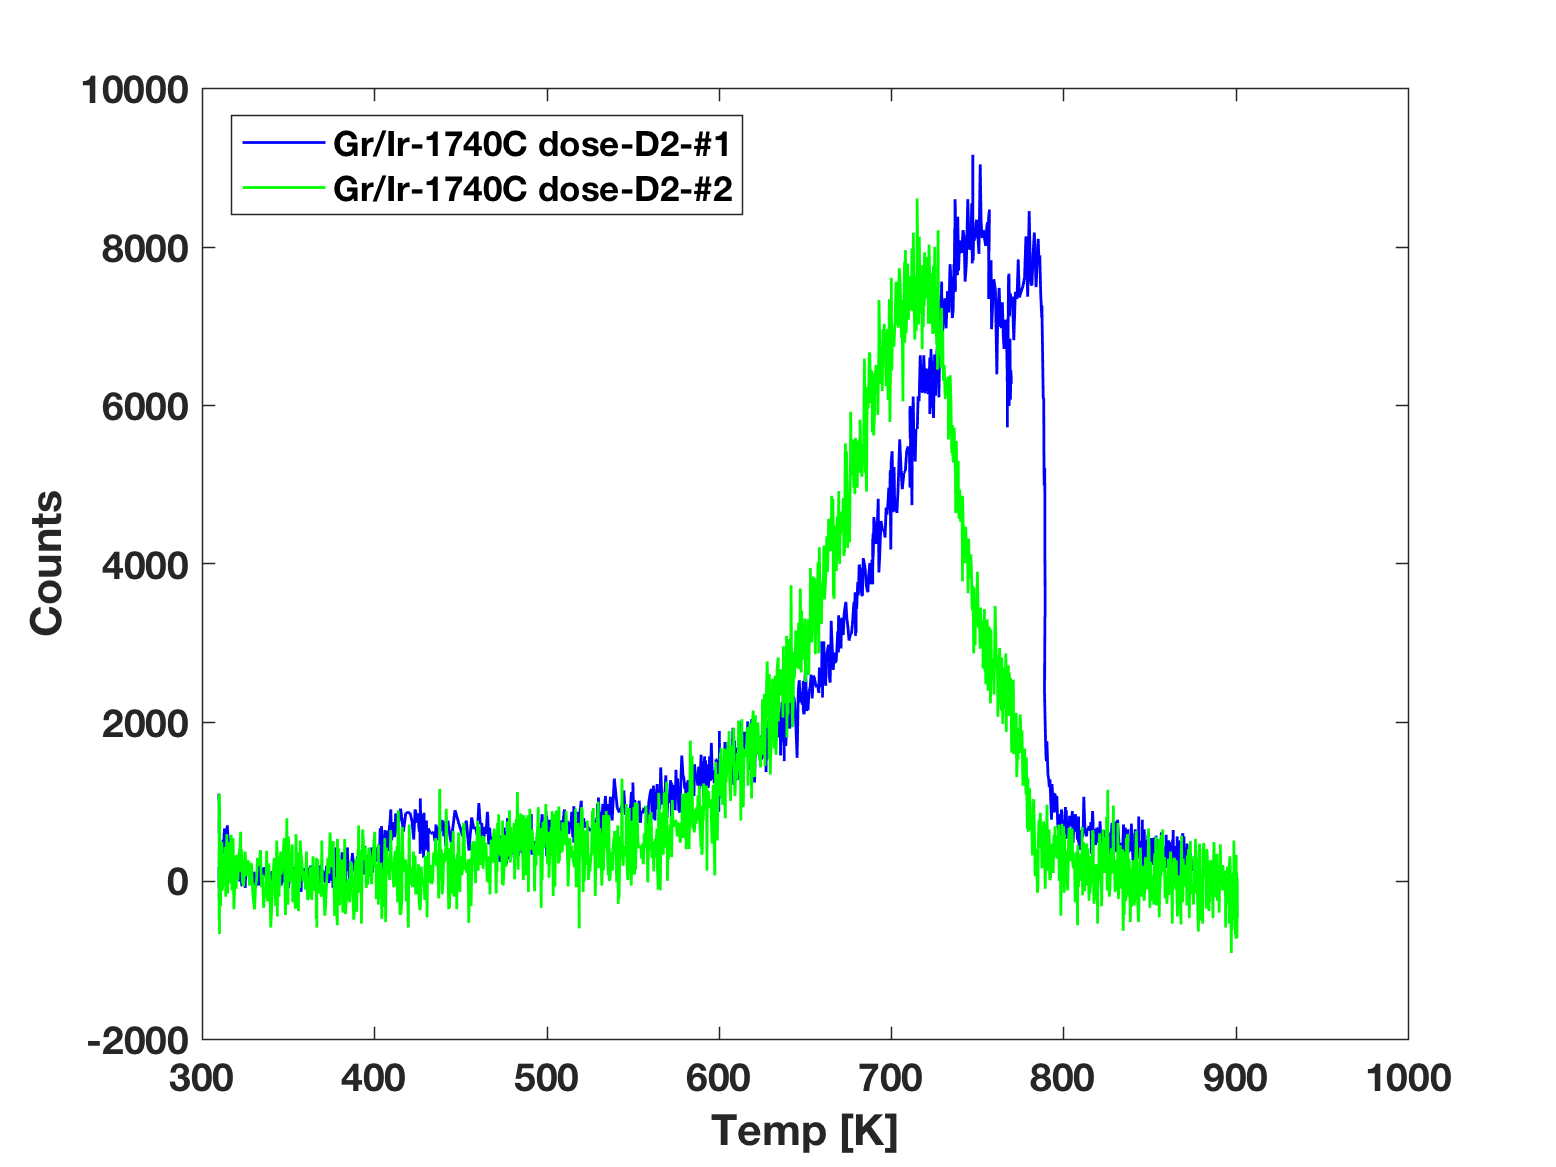
\includegraphics[width=\textwidth]{TPD/050516IrSorenD2dose1hourtemp.png}
    \caption{}
    \label{TPD:D22}
  \end{subfigure}\hspace{0.5cm}
  \begin{subfigure}[b]{0.45\textwidth}
    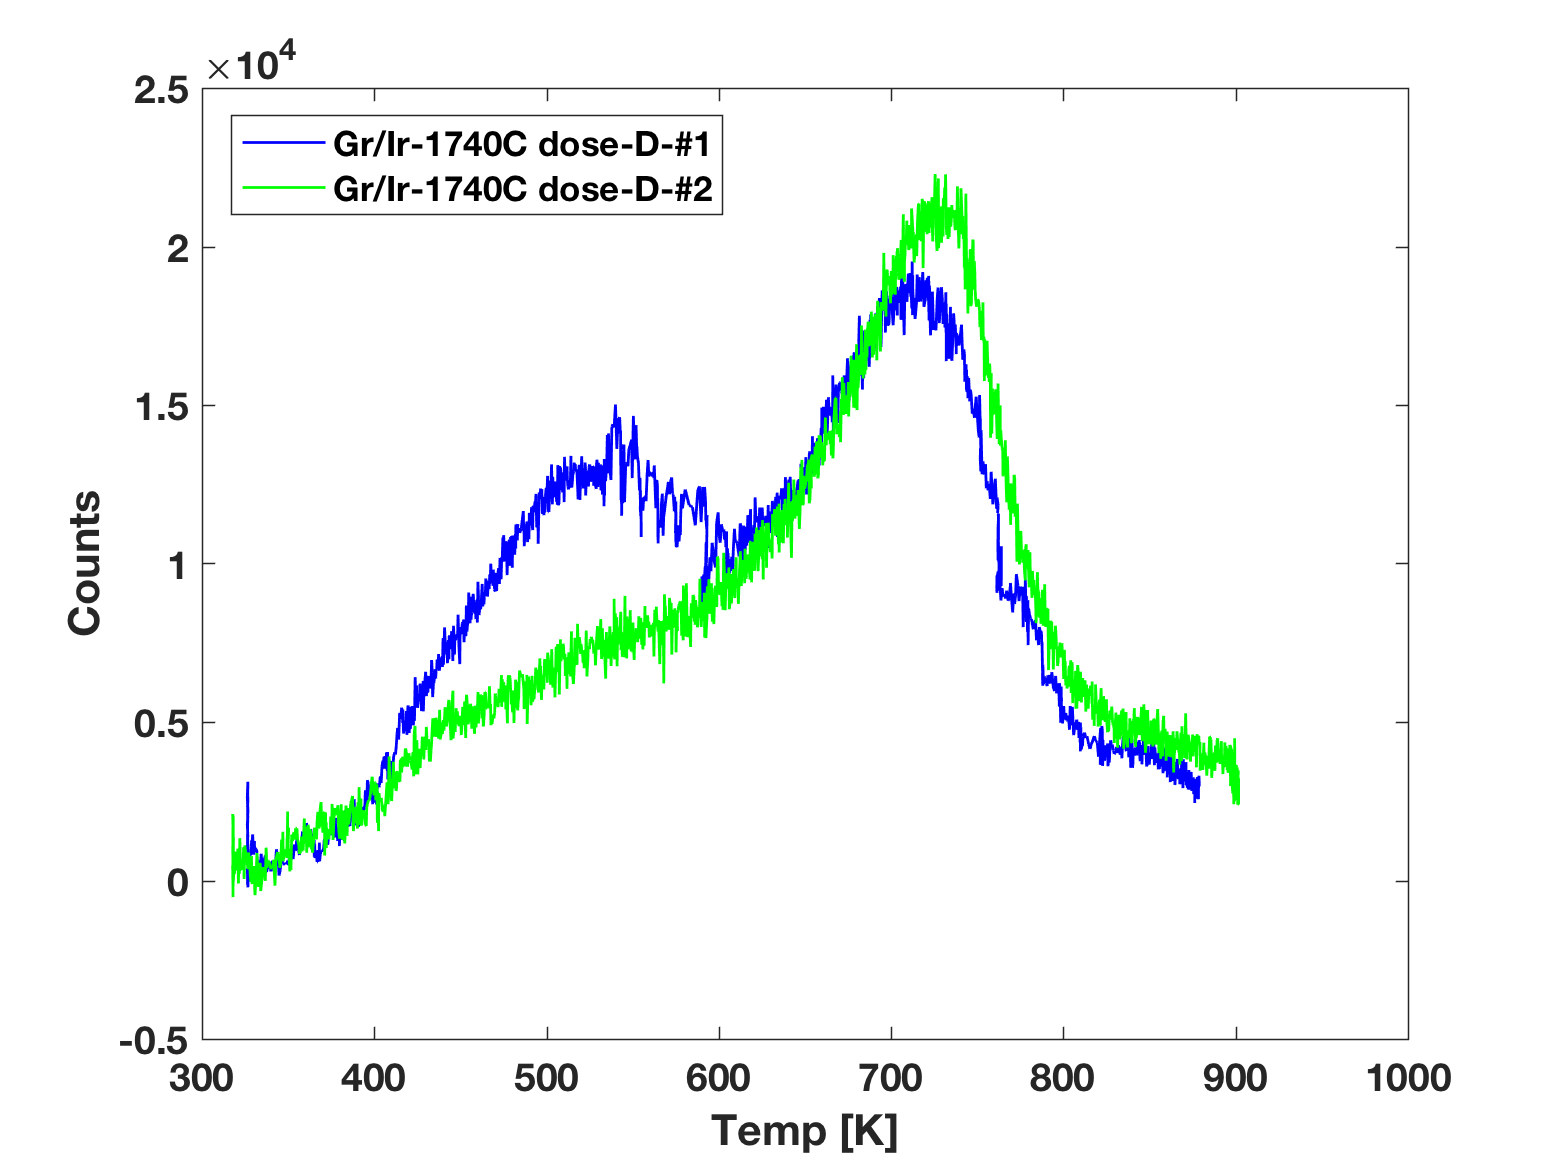
\includegraphics[width=\textwidth]{TPD/050516IrSorenDdose1hourtemp.png}
    \caption{}
    \label{TPD:D2}
  \end{subfigure}
  \caption{TPD measurements following doses of D$_2$ and atomic hydrogen. (a) shows the graph following a 1 hour D$_2$ dose on graphene on Ir(111) with a doser temperature of 1740 \degree C and a chamber pressure of $5\cdot 10^{-7}$mbar. and (b) shows the graph following a 1 hour D dose on graphene on Ir(111) with a doser temperature of 1740 \degree C and a chamber pressure of $5\cdot 10^{-7}$mbar.}
  \label{TPD:all}
\end{figure}


\subsection{STM images of bilayers}

In the following section STM images of bilayer patches are included. These images are made prior to the long anneal, and are therefore not directly related to the experiment mentioned in the preceding section. It was not possible to make images of the sample after the long anneal in ethylene, since the STM was broken. Bilayers were however present on the surface prior to the long anneal, and the following images show some of the key points about these.\\
The images in figure \ref{D2:} are made after the 12 hour dose of hydrogen at a chamber pressure of $1\cdot 10^{-5}$mbar with the ion gauge turned on. Hence the surface is fully hydrogenated which is somehow different to see due to the large images. On figure \ref{D2:bilayer1}, the three-point-star-structures characteristic for the hydrogenated surface are however seen, which is pointed out with the blue arrows. Bilayer patches are seen on the top half of the figure, and none of the structures characteristic for the fully hydrogenated surface are seen. A new superstructure is however seen with the individual flower-like structures, with a center circle surrounded by six other circles, construct a bigger pattern.\\
On figure \ref{D2:bilayer2} a linescan was made across the edge of the graphene monolayer-bilayer edge. The corresponding line profile is shown in figure \ref{linescanbilayer1}, and from this the height difference is measured to 2.97 $\pm$ 0.5Å. The bilayer edge is therefore significantly higher than the Iridium step edge, and much closer to the layer height of HOPG which is 0.35nm.\cite{PhysRevB.79.195429}\\
In order to investigate the bilayer superstructure further, a zoom in of figure \ref{D2:bilayer2} was made as seen in figure \ref{D2:bilayer3}. The graphene sheet is seen due to the atomic resolution, and it is obvious that no hydrogen is adsorbed to the surface. This is consistent with the data from the TPD measurements. Furthermore it is seen that the consistency in the superstructure is absent. Some areas of the bilayer has a cluster of three circles forming a triangle that points either up or down. These are highlighted in the left side of the picture. Other areas seem to have the flower-like structure mentioned earlier, but with an overlapping hexagon. An attempt to determine the periodicity of the superstructure was done by doing a linescan between two identical parts of the pattern. As seen on figure \ref{D2:bilayer3} the linescan was drawn between two down facing triangles, and the distance between these were measured from the bottom corner. The line profile is shown in figure \ref{linescanbilayer2} and the length between the points is measured to 45.78 $\pm$ 1Å.

\begin{figure}[H]
\makebox[\textwidth][c]{
  \begin{subfigure}[b]{0.3\paperwidth}
    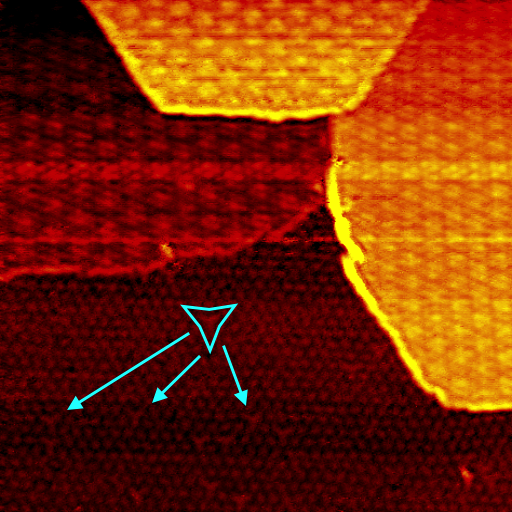
\includegraphics[height=\textwidth]{STMdata/FFT/2016-04-13_001_49.png}
    \caption{940x940 Å - I$_t$ = 0.850 nA, V$_t$ = 75.7 mV}
    \label{D2:bilayer1}
  \end{subfigure}
  \begin{subfigure}[b]{0.3\paperwidth}
    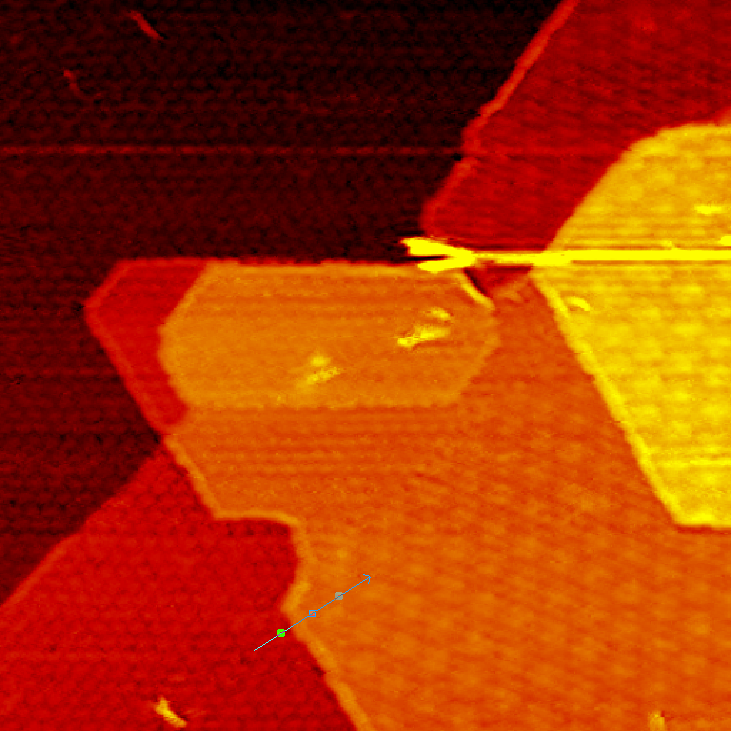
\includegraphics[height=\textwidth]{STMdata/FFT/2016-04-13_001_50.png}
    \caption{928x928Å - I$_t$ = 0.800 nA, V$_t$ = 75.7 mV}
    \label{D2:bilayer2}
  \end{subfigure}
  \begin{subfigure}[b]{0.3\paperwidth}
    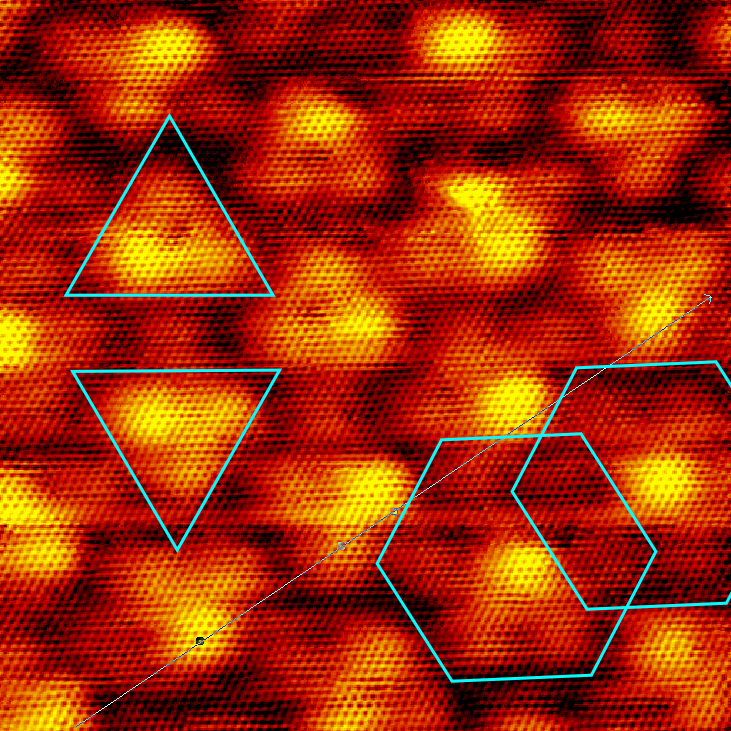
\includegraphics[height=\textwidth]{STMdata/FFT/2016-04-13_001_55.png}
    \caption{196x196 Å - I$_t$ = 0.820 nA, V$_t$ = 75.7 mV}
    \label{D2:bilayer3}
  \end{subfigure}
}
\\
\makebox[\textwidth][c]{
\begin{subfigure}[b]{0.35\paperwidth}
  \includegraphics[width=\textwidth]{STMdata/FFT/linescanbilayer1}
  \caption{Line profile belonging to the linescan in (b)}
  \label{linescanbilayer1}
\end{subfigure}
\begin{subfigure}[b]{0.35\paperwidth}
  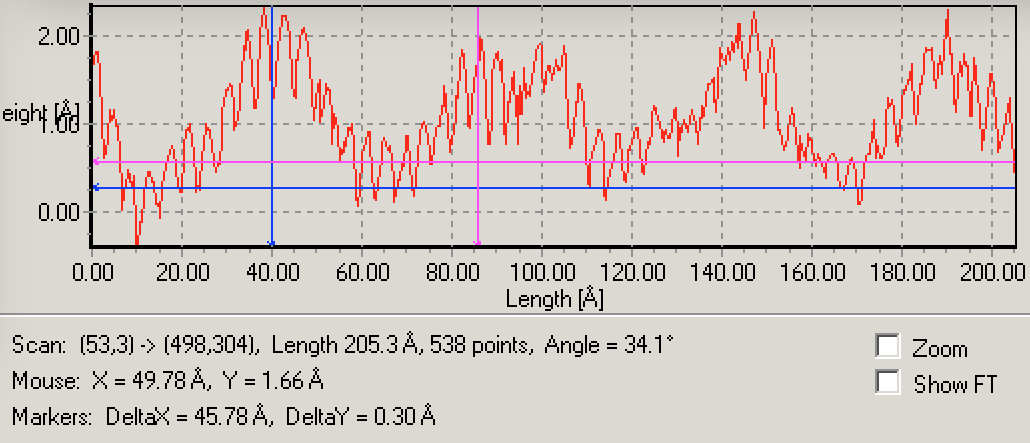
\includegraphics[width=\textwidth]{STMdata/FFT/linescanbilayer2}
  \caption{Line profile belonging to the linescan in (c)}
  \label{linescanbilayer2}
\end{subfigure}
}
\caption{Patches of bilayered graphene on Ir after a hydrogen dose at $1\cdot 10^{-5}$mbar for 12h.}
\label{D2:bilayer}
\end{figure}


\subsection{LEED of bilayered sample}
LEED was performed on the sample after an ethylene anneal with a chamber pressure of $7\cdot 10^{-7}$mbar. The figures in \ref{LEED} show pictures of the fluorescent screen within the UHV chamber from which the LEED was performed. The image on figure \ref{LEED1} shows the fluorescent screen after the untreated sample was exposed to an electron beam with an energy of 145eV. The spots marked out with the marked arrows show the diffraction pattern from the underlying Ir(111) surface, as well as the graphene sheet on top of the surface.\cite{1367-2630-10-4-043033}\\
The sample was then flashed to a low temperature in order to maintain any bilayers, and the sample was once again exposed to an electron beam of energy 145eV. The top and bottom right corner of the hexagonal pattern is enlarged in figure \ref{LEED2}. From this figure it is clear that some extra spots appear around the Ir and C spots pointed out in the previous figure. These spots arise from the moiré pattern of the graphene on Ir(111) surface. The reason why these spots were absent in the previous figure might be caused by a high amount of contaminants on the surface. These ruin the periodicity of the surface, and hence also the electron scattering, which then becomes smeared out. After annealing to a low temperature these contaminants should be gone, leaving the surface clean with small patches of bilayered graphene. The patches of bilayered graphene should however also cause a different scattering due to the changed periodicity as seen in figure \ref{D2:bilayer3}. If figure \ref{LEED2} and \ref{LEED3} is compared it does look like the spot belonging to the carbon atoms and the surrounding moiré spots in figure \ref{LEED2} are less distinct. These results might therefore indicate that bilayers are present on the surface in figure \ref{LEED2} and to a lesser extent in figure \ref{LEED3}. Since the picture in figure \ref{LEED3} is taken prior to an 1090\degree C anneal, it is reasonable to conclude that the bilayer patches desorb from the surface when annealing to this temperature.[Reference til desorption af bilayers?]

\begin{figure}[H]
\makebox[\textwidth][c]{
  \begin{subfigure}[b]{0.3\paperwidth}
    \includegraphics[height=\textwidth]{LEED/No" "flash/145eV.JPG}
    \caption{LEED without flashing. 145eV.}
    \label{LEED1}
  \end{subfigure}
  \begin{subfigure}[b]{0.3\paperwidth}
    \includegraphics[height=\textwidth]{LEED/Low" "T" "flash/145eV.JPG}
    \caption{LEED after low T flash. 145eV}
    \label{LEED2}
  \end{subfigure}
  \begin{subfigure}[b]{0.3\paperwidth}
    \includegraphics[height=\textwidth]{LEED/post" "1090" "flash/145eV.JPG}
    \caption{LEED after 1090\degree C flash. 145eV}
    \label{LEED3}
  \end{subfigure}
}
\caption{LEED pictures from the Gr/Ir sample with bilayers. [Reference til Antonija/Hoffmanlab]}
\label{LEED}
\end{figure}
